\definecolor{codegreen}{rgb}{0,0.6,0}
\definecolor{codegray}{rgb}{0.5,0.5,0.5}
\definecolor{codepurple}{rgb}{0.58,0,0.82}
\definecolor{backcolour}{rgb}{0.95,0.95,0.92}

\lstdefinestyle{configstyle}
{
	backgroundcolor=\color{backcolour},   
	commentstyle=\color{codegreen},
	keywordstyle=\color{red},
	numberstyle=\tiny\color{codegray},
	stringstyle=\color{codepurple},
	basicstyle=\footnotesize,
	breakatwhitespace=false,         
	breaklines=true,                 
	captionpos=b,                    
	keepspaces=true,                 
	numbers=left,                    
	numbersep=5pt,                  
	showspaces=false,                
	showstringspaces=false,
	showtabs=false,                  
	tabsize=2
}


\chapter{Docker}
\section{Geschiedenis van Containers}
%TODO bron docker relases invoegen
%TODO chroot bron: http://www.faqs.org/faqs/unix-faq/faq/part6/section-2.html
%TODO what chroot does: http://man7.org/linux/man-pages/man2/chroot.2.html
Docker op zich bestaat nog niet zo lang. Versie 0.1.0 is uitgekomen op 26 maart 2016 en versie 1.0.0 en dus de eerste effectieve release kwam uit op 9 juni 2014. Hierdoor is er nog niet veel geschiedenis aan Docker. Maar als we terugkijken naar de evolutie van containers gaat dit verder terug. 
Het idee van containers gaat terug tot 1979 met de toevoeging van chroot in UNIX V7. chroot is een eerste concept van containerization. Hierbij wordt voor elk proces een geisoleerde ruimte op de schijf voorzien, ook wel een "chroot jail" genoemd.
%TODO http://imesh.io/evolution-of-linux-containers-and-future/
Na chroot duurde het tot het jaar 2000 tot het volgende op de markt kwam. FreeBSD Jails(2000) en Linux VServer(2001) waren beide jail mechanismen die verder bouwden op chroot. Hiernaa kwamen enkele oplossingen op de markt die al dichter bij de container die we nu kennen aansluiten namelijk Solaris Containers(2004), OpenVZ(2005), Process Containers(2006) en Control Groups(2007).

Daarna werd in 2008 LXC (LinuX Containers) toegevoegd aan de linux kernel. Dit was de basis voor latere containerizatie technologieën. LXC cobineerde het gebruik van cgroups (dit stond in voor isolatie en resource management) en namespaces (dit zorgde ervoor dat groups opgesplitst konden worden waardoor ze elkaar niet kunnen "zien")\cite{Ellingwood2015}.In 2014 werd de versie 1.0 van LXC uitgebracht. Hierbij werd onder andere support toegevoegd voor SELinux. De eerste versies van Docker waren ontwikkeld als een interne tool bij het bedrijf dotCloud. Deze tool zorgde voor een versimpeling voor het gebruik van LXC. Later werd dit uitgebracht onder de naam Docker een 	en werd de LCX container vervangen door hun eigen driver LibContainer. Docker zorgde als een van de eerste voor een volledig ecosysteem voor het managen van containers \cite{Gunaratne2016}.
 
\section{Wat is Docker}

Docker is een open source project om een applicatie te verpakken, verzenden en te draaien als een weinig resources gebruikende container. Anders gezegd word in een Docker Container alles om een programma te draaien verpackt in een compleet bestandsysteem namelijk: code, runtime, stysteem tool en systeem librairies. Alles wat je normaal op een server zou installeren. Dit garandeerd dat de applicatie zich altijd op dezelfde manier zal gedragen in welke omgeving het ook draait \cite{Docker2016d}.

Een vergelijking met virtuele machines is rap gemaakt. Voor resource isolatie werkt het op dezelfde manier. Maar waar de verschillen liggen is de grootte, flexibiliteit en performatie. Doordat Docker gebruik maakt van containerization gebeurt de virtualizatie op de kernel niveau tegenover virtuele machines waarbij dit niet zo is. 

\begin{figure}[!ht]
	\centering
	\begin{minipage}{.5\textwidth}
		\centering
		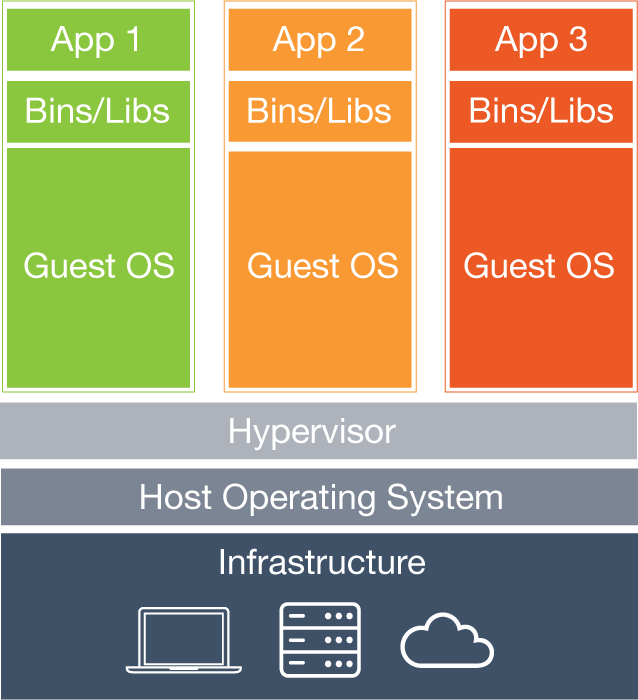
\includegraphics[width=.7\linewidth]{img/what-is-docker-diagram.png}
		\caption{Virtualisatie bij Virtuele machines- \protect\cite{Docker2016d}}
		\label{fig:test1}
	\end{minipage}%
	\begin{minipage}{.5\textwidth}
		\centering
		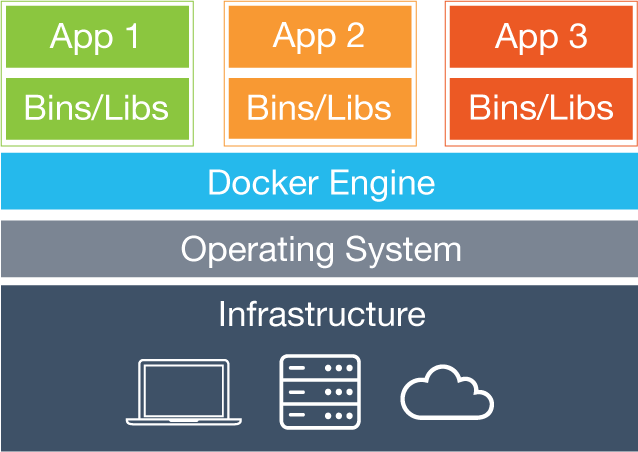
\includegraphics[width=.7\linewidth]{img/what-is-vm-diagram.png}
		\caption{Virtualisatie bij Docker Containers - \protect\cite{Docker2016d}}
		\label{fig:test2}
	\end{minipage}
\end{figure}

Een korte visualisatie van hoe containers werken kunnen we zien op de voorgaande foto's. Hierbij zien we dat traditioneel bij virtuele machines we op de host die zich rechtstreeks bevind op de hardware een hypervisor nodig hebben die onze hardware gaat virtualiseren voor gebruik van de virtuele gast machines. Op elke gast machine bevind zich een eigen besturingssysteem die uniek is voor elke gast. Daarnaast moeten ook onze applicatie draaien samen met de binaries en librairies die het nodig heeft. Bij containerisatie en specifiek voor docker containers wordt de hypervizor vervangen door de docker engine en gaan we voor elke applicatie onze binaries en libraries samen met de applicatie zelf gaan draaien in onze container. Hierdoor krijgen we snellere deployment, opstart tijden en migratie en daarnaast hebben we ook veel minder overhead doordat niet ekle applicatie moet draaien op een eigen besturingssysteem en een eigen kernel. 

\section{Hoe gebruikt men Docker}

Doordat in deze bachelorproef zeer veel met docker gewerkt wordt en het relatief nieuwe software is zal ik in deze sectie uitleggen hoe men zelf met docker aan de slag kan. Het basis gebruik van docker is bewust simpel gehouden. Maar we mogen niet vergeten dat we over een krachtige en flexibele tool beschikken waardoor we docker ook complex kunnen maken.

\subsection{installatie}

De installatie van docker kan op verschillende manieren. Een van deze manieren is met het 'curl' commando. Daarnaast beschikt Docker ook over een 'apt' en 'yum' repository. Installatie met de package managers voor 'apt' en 'yum' doen we met 'sudo apt-get install Docker' en 'sudo yum install Docker' respectievelijk. Voor de installatie met 'curl' gaan we uit van een Ubuntu systeem maar kan ook uitgevoerd worden met een andere package manager op een ander linux besturingssysteem. Een eerste stap is de installatie van 'curl' zelf. Hiervoor kijken we eerst als we 'curl' al geïnstalleerd hebben. 'sudo wich curl' geeft ons de geïnstalleerde versie van 'curl'. Indien het not niet geïnstalleerd is kunnen we met 'sudo apt-get update' en 'sudo apt-get install curl' het installeren. Deze stap kan op andere besturingssystemen uitgevoerd worden met de package manager van dat besturingssysteem. In veel besturingssysteem wordt curl al megeleverd van de manufacturer. Daarna kunnen we het commando 'curl -fsSL https://get.docker.com/ | sh' uitvoeren. Dit zal Docker downloaden en installeren. Dit is op de vershillende besturingssystemen hetzelfde. Als we Docker installeren via een user moeten we er rekening mee houden dat we de deze user root rechten geven, meer hierover in het hoofdstuk over security. Na het installeren van Docker kunnen we met het commando 'docker run hello-world' nagaan of onze installatie gelukt is. Indien de installatie succesvol was moeten we nu samen met nog andere output het bericht 'Hello from Docker. This message shows that your installation appears to be working correctly.' krijgen.

%TODO insert text line for docker run hello-world

\subsection{docker images}

Wanneer we images gebruiken hebben we twee opties. Aan de ene kant kunnen we de docker images van een repository gebruiken (bvb. de Docker hub) aan de andere kant hebben we ook de optie om onze eigen images te maken. 

\paragraph{Docker images van een repository}~\\

In dit voorbeeld gaan we de Docker hub repository gebruiken. Dit is de officiële repository van Docker. Iedereen kan images uploaden naar de Docker hub. Het enige dat daarvoor benodigd is, is een Docker hub account. Om te kijken welke Images er beschikbaar zijn hebben we 2 opties. Ofwel kijken we op de website van docker hub (hub.docker.com). Hier kunnen we met behulp van de search bar (zie image) Docker images zoeken. We kunnen dit ook direct van de command line. Dit doen we met het commando 'docker search ZOEKTERM', hierbij doorzoeken we alle geïnstalleerde registries op onze machine (standaard is dit enkel de Docker hub). Om een voorbeeld te geven gaan we op zoek naar een image genaamd 'docker-alpine-redis' het resultaat van deze zoekopdracht volgens de twee voorgaande methodes kunt u vinden in de volgende figuren.
\begin{figure}[!ht]
	\centering
	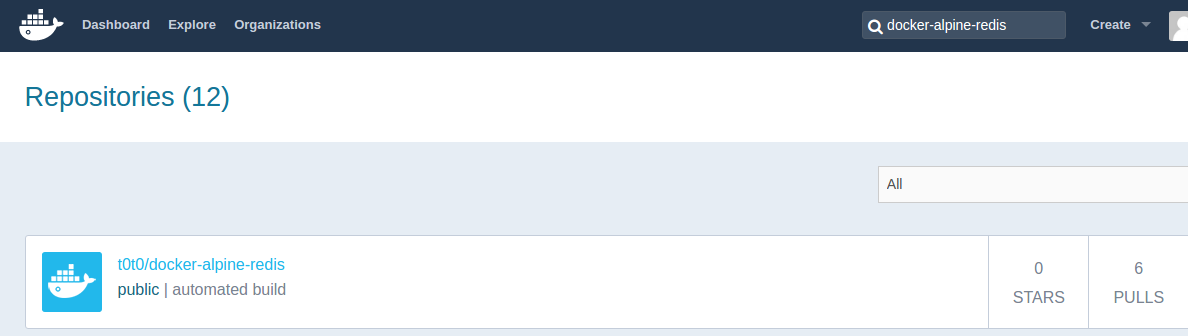
\includegraphics[scale=0.315]{img/dockerSearchSite.png}
	\caption{Zoeken naar images op de docker hub site}
\end{figure}

\begin{figure}[!ht]
	\centering
	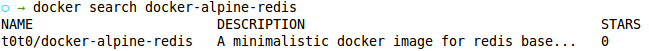
\includegraphics[scale=0.55]{img/dockerSearchCommand.png}
	\caption{Zoeken naar images via command-line}
\end{figure}	




\paragraph{Eigen Docker images maken}~\\

Naast het gebruik van de Docker hub kunnen we ook onze eigen images maken die we desgewenst kunnen uploaden naar de Docker hub. Het maken van een docker image begint bij een Dockerfile. In deze Docker file definiëren we hoe onze container er moet uitzien wanneer we de image inladen in die container. Een eerste stap is het aanmaken van een map waarin we gaan werken. Deze map is de context die naar de docker daemon wordt gestuurd om de image te maken, dit wil zeggen dat de docker deamon die de image gaat maken voor ons niet buiten deze folder kan op zoek gaan naar files die we willen toevoegen. Dus alle files die we willen toevoegen aan onze image moeten we in deze folder plaatsen. na het aanmaken van deze map voegen we er een file genaamd 'Dockerfile' (case sensitive) aan toe. Een voorbeeld van zo een 'Dockerfile' vinden we hieronder. 

\begin{lstlisting}[language=bash, style=configstyle]
# Base image alpine
FROM alpine:3.3

MAINTAINER Tomas Vercautter & Toon Lamberigts

# Environment varabelen
ENV REDIS_VERSION=3.0.7
ENV REDIS_IMAGE=redis-$REDIS_VERSION
ENV REDIS_IMAGE_TAR=$REDIS_IMAGE.tar.gz
ENV REDIS_DOWNLOAD_URL=http://download.redis.io/releases/$REDIS_IMAGE_TAR

# Install redis en dependencies
RUN apk --no-cache add --virtual .dependencies \
    make \
    gcc \
    wget \
    linux-headers \
    musl-dev \
    tcl \
    tar && \
    wget "$REDIS_DOWNLOAD_URL" && \
    tar xzf $REDIS_IMAGE_TAR && \
    cd $REDIS_IMAGE && \
    make && \
    cp src/redis-server /usr/bin/ && \
    cp src/redis-cli /usr/bin/ && \
    rm -r /$REDIS_IMAGE && \
    rm -r /$REDIS_IMAGE_TAR && \
    apk del .dependencies && \
    rm -rf /var/cache/apk/* && \
    mkdir /data

# Commando die wordt uigevoerd bij het starten van container
CMD redis-server --dir /data --appendonly yes

# Expose de poort voor redis
EXPOSE 6379
\end{lstlisting}

In deze Dockerfile zien we een aantal sleutelwoorden in het rood. deze zijn de verschillende elementen van de Dockerfile. Docker images kunnen gebaseerd zijn op andere Docker images. Dit wordt gedefinieerd met het sleutelwoord 'FROM' hier kan je zien dat deze image gebaseerd is op een 'alpine' images, meerbepaald de image met tag '3.3'. Het volgende sleutelwoord dat we tegenkomen is 'MAINTAINER' dit voegt aan de image info een 'author' tag toe. Dit kunnen we zien met 'docker inspect NAME'. Dit toont ons alle informatie over de container of image gedefinieerd met 'NAME'. Het 'MAINTAINER' sleutelwoord geeft verder geen invloed op de werking van de image. Daarna komen we het 'ENV' sleutelwoord tegen. Hiermee kunnen we environment variabelen declareren voor de image. Dit wordt vaak gebruikt om versies van software aan te duiden waardoor de Dockerfile makkelijker leesbaar blijft. Het 'RUN' sleutelwoord duid aan welke commando's uitgevoerd worden bij het aanmaken van de image. Dit zijn de commando's die normaal zouden uitgevoerd worden bij het installeren van de gewenste software. In dit geval installeren we redis dus hebben we eerst de dependencies voor het installeren van redis in een groep geïnstalleerd waardoor we die later kunnen verwijderen als groep. Hierna wordt redis gedownload van de officiële site, uitgepakt en geinstalleerd. Na de installatie ruimen we alles op om de image zo klein mogelijk te houden. Dan hebben we twee sleutelwoorden die het runnen van de container makkelijker maken, namelijk 'CMD' en 'EXPOSE'. 'CMD' zorgt ervoor dat het commando dat erna komt uigevoerd wordt wanneer we een container met deze image opstarten en 'EXPOSE' zet een poort van de container, in dit geval 6379, open. Door deze twee sleutelwoorden moeten we de twee overeenstemmende opties niet meer meegeven in ons run commando.

Het creëren van een image uit een Dockerfile doen we met het docker build commando doen we met het commando 'docker build [OPTIONS] PATH' waarbij de 'PATH' wordt vervangen door het pad (relatief of absoluut) naar de buildcontext die zal worden meegegeven naar de docker daemon voor het builden van de image. In ons geval is dit de map die we daarnet hebben aangemaakt. De Docker daemon zal an op zoek gaan in de root van de buildcontect naar een Dockerfile en de met sleutelwoorden gedefinieerde commando's uitvoeren en een Docker image maken van onze Dockerfile. Indien de dockerfile niet in de root van onze buildcontext bevindt kunnen we met de optie '-f' een relatief pad naar onze Dockerfile toevoegen. Met de optie '-t' kunnen we een eigen tag meegeven aan onze image. Dit helpt ons met het identificeren welke image wat is. In ons voorbeeld met de Dockerfile voor redis is het commando 'docker build -t redis .' indien we ons in de map met de Dockerfile bevinden. Na het uitvoeren van het commando hebben we een image genaamd redis gemaakt met onze Dockerfile. Dit kunnen we controleren met het 'docker images' commando. Dit geeft ons een lijst met alle images die zich lokaal op onze machine bevinden. In ons geval geeft dit de volgende output. Hierop kunnen we zien dat de image voor 'alpine:3.3' is gedownload doordat we dit als base image hebben gedefineerd en dat onze 'redis' image is aangemaakt.


\begin{figure}[!ht]
	\centering
	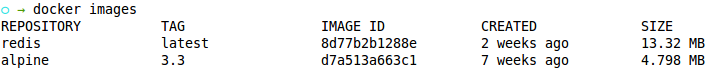
\includegraphics[scale=0.55]{img/dockerImages.png}
	\caption{Output van het docker images commando}
\end{figure}



\subsection{docker run}

Met het 'docker run [OPTIONS] IMAGE[:TAG|@DIGEST] [COMMAND] [ARG...]' commando kunnen we een image naar keuze inladen in een container. Het basis commando hebben we al eerder gebruikt met 'docker run hello-world' dit neemt de Docker image 'hello-world' en laad deze in een container waardoor ze kan interageren het environment. Bij het uitvoeren van het 'docker run' commando kunnen we zowel een locale image als een image uit een repository kiezen. Om een image te kiezen van uit een repository moeten we niets extra doen. De docker software kijkt bij het uitvoeren van het commando eerst als we image lokaal hebben. Indien dit het geval is wordt de image in een container geladen en opgestart. Indien dit niet het geval is zoekt de docker software naar te image in de voorgedefinieerde repositories (standaard enkel docker hub) en als het de gekozen image vind wordt het gedownload en ingeladen en opgestart.

Daarnaast kunnen we ook opties meegeven aan het run commando. Hiermee kunnen we volumes mounten met de '-v' optie, extra poorten exposen die nog niet in de image gedefinieerd zijn met '--expose', poorten van de container mappen op poorten van de host met de '-p' optie, een naam megeven aan onze container met de optie '--name'  of de container detached laaten draaien met de optie '-d' indien we dit niet meegeven wordt de container attached aan ons terminal venster en kunnen we het voor niets anders meer gebruiken. Dit zijn slechts enkel voorbeelden van opties die we hebben de rest van de opties zijn te vinden in de docker run reference (TODO INSERT LINK TO REFERENCE BIJLAGE?). Ook kunnen we commando's meegeven bij het runnen van een container. Het meegegeven commando wordt uitgevoer als we de container opstartn. Er moet altijd een commando meegegeven worden als we een container willen starten maar dit kan ook worden meegegeven in de image. Als voorbeeld zullen we de redis image dat we daarnet hebben gemaakt laden in een container. Hiervoor gebruiken we het commando 'docker run -d --name redisContainer redis'. Dit maakt van onze image genaamd redis een container genaamd redisContainer die detached draait. Om te controleren als onze container nu draait gebruikten we het commando 'docker ps' dit geeft ons een lijst van alle draaiende containers op onze machine. 
 
 
\begin{figure}[!ht]
 	\centering
 	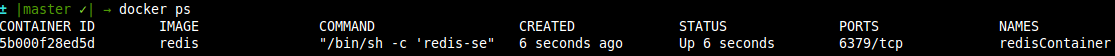
\includegraphics[scale=0.35]{img/dockerps.png}
 	\caption{Output van het docker ps commando}
\end{figure}